\clearpage
\section{Background}

% ********************************************************************************
% ********************************************************************************
% ********************************************************************************

\subsection{Object Detection}
\label{sec:object-detection}

\textit{TODO: introduce topic}

State of the art visual road defects detection rely on object detection. Object detection is the combination of classifying and locating the object. The output of the model is the detected class and the bounding box where that object is detected. Within a single image there can be one or multiple defects, sometimes from different types. With object detection it is possible to locate all these different instances. Object detection is well researched topic. The most commonly referred models are known as R-CNN, Fast R-CNN, Faster R-CNN and YOLO.


\subsubsection{R-CNN}
A naive approach to solve the problem of localizing objects is to slide a window over the image, and for each window perform classification. However the problem with this approach is that objects may have different location, sizes and aspect ratios. To make this work, an infinite possibility of regions need to be computed. 

\authorref{Girshick2013} solves this problem by proposing a model called Regions with CNN (R-CNN). Their approach is to extract 2000 regions using a region proposal algorithm (in paper they use selective search). For each region they use a CNN to extract features and SVM to make the classification. 

\begin{figure}[ht]
\begin{center}
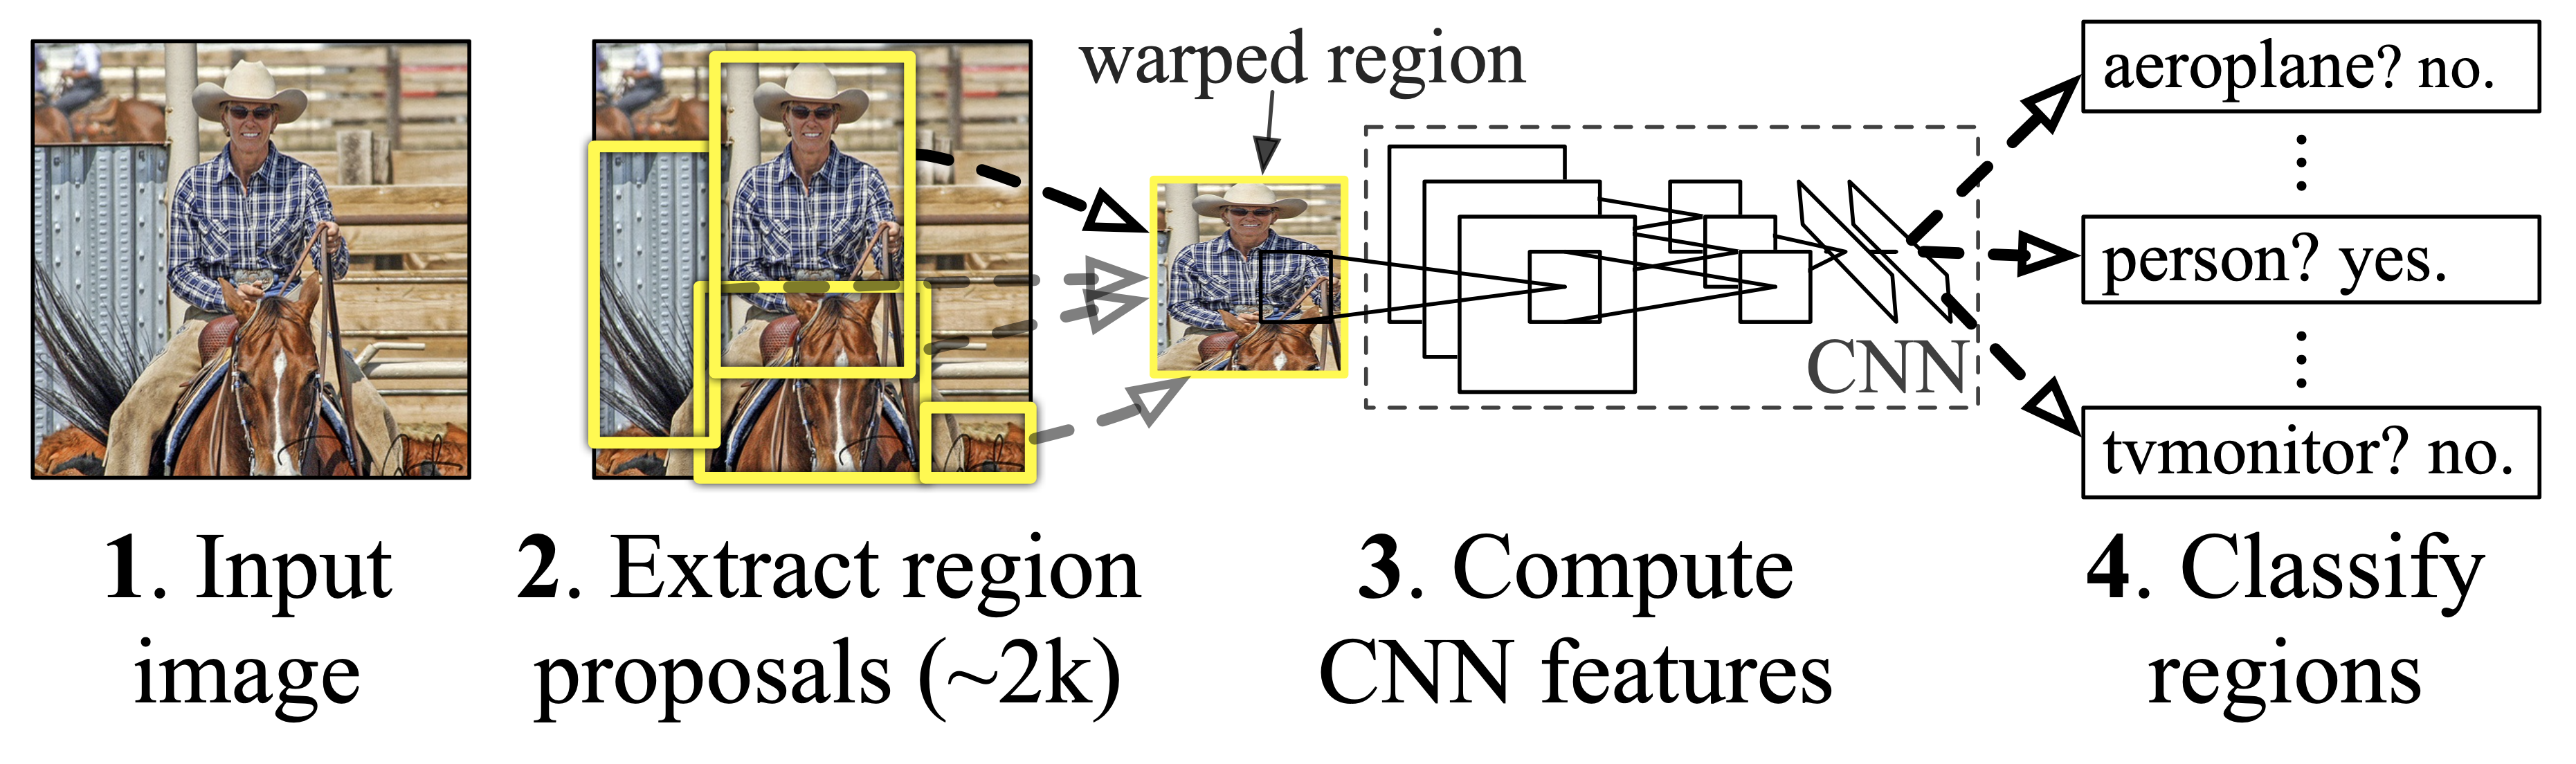
\includegraphics[height=2cm,keepaspectratio]{images/2_literature/r-cnn.png}
\end{center}
\caption{R-CNN: Object detection overview \cite{Girshick2013}.}
\end{figure}

\subsubsection{Fast R-CNN}
Drawback of the method above has some drawbacks. Mainly it is slow because it performs a CNN for each of the 2000 object proposals. The author\authorref{Girshick2015} continued its work to solve this problem. With the new proposed model called Fast R-CNN. This novel model can detect object in an image in 2 seconds, whereas the original R-CNN takes about 50 seconds per image.

Instead of feeding each of the proposed regions to the CNN, the Fast R-CNN takes as input the entire input image and proposed regions. From the output, regions of interests are identified and are fed into fully connected layers to output the class and location of the object. 

\begin{figure}[ht]
\begin{center}
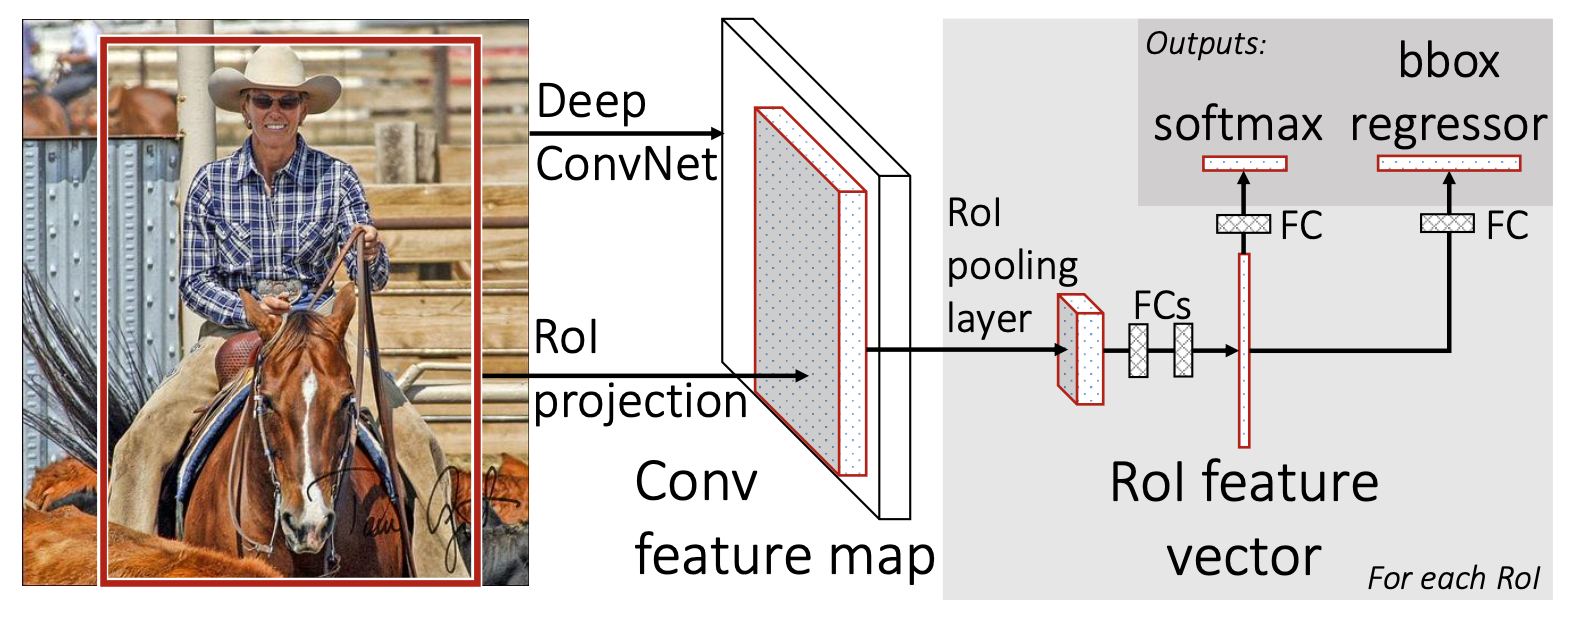
\includegraphics[height=2cm,keepaspectratio]{images/2_literature/fast-r-cnn.png}
\end{center}
\caption{Fast R-CNN: Object detection overview \cite{Girshick2013}.}
\end{figure}

\subsubsection{Faster R-CNN}
Although Fast R-CNN is significantly quicker to detect objects, it still takes about 2 seconds to localize the object. The bottleneck is the region proposal algorithm, which is implemented on the CPU. Improvements over the used selective search were researched. However, \authorref{Ren2015} argued that it would be interesting to implement a model which combines region proposal and object detection. Their model was called Faster R-CNN and is able to process an image in 200 milliseconds. 

Faster R-CNN consists of two modules. The first module is a deep fully convolutional network which proposes regions, known as Region Proposal Network (RPN). The RPN takes an image as input and outputs a set of object proposals, each with an \textit{objectness score} (measurement if something is an object or background). This output is fed into the second module, which is the Fast R-CNN object detector. 

The unified model has several advantages over the Fast R-CNN model. Because the region proposal are generated within the network, the model can be trained end-to-end. Making usage easier and requires less resources. Additionally, this allows the region proposals to be tuned according to the detection task.


\begin{figure}[ht]
\begin{center}
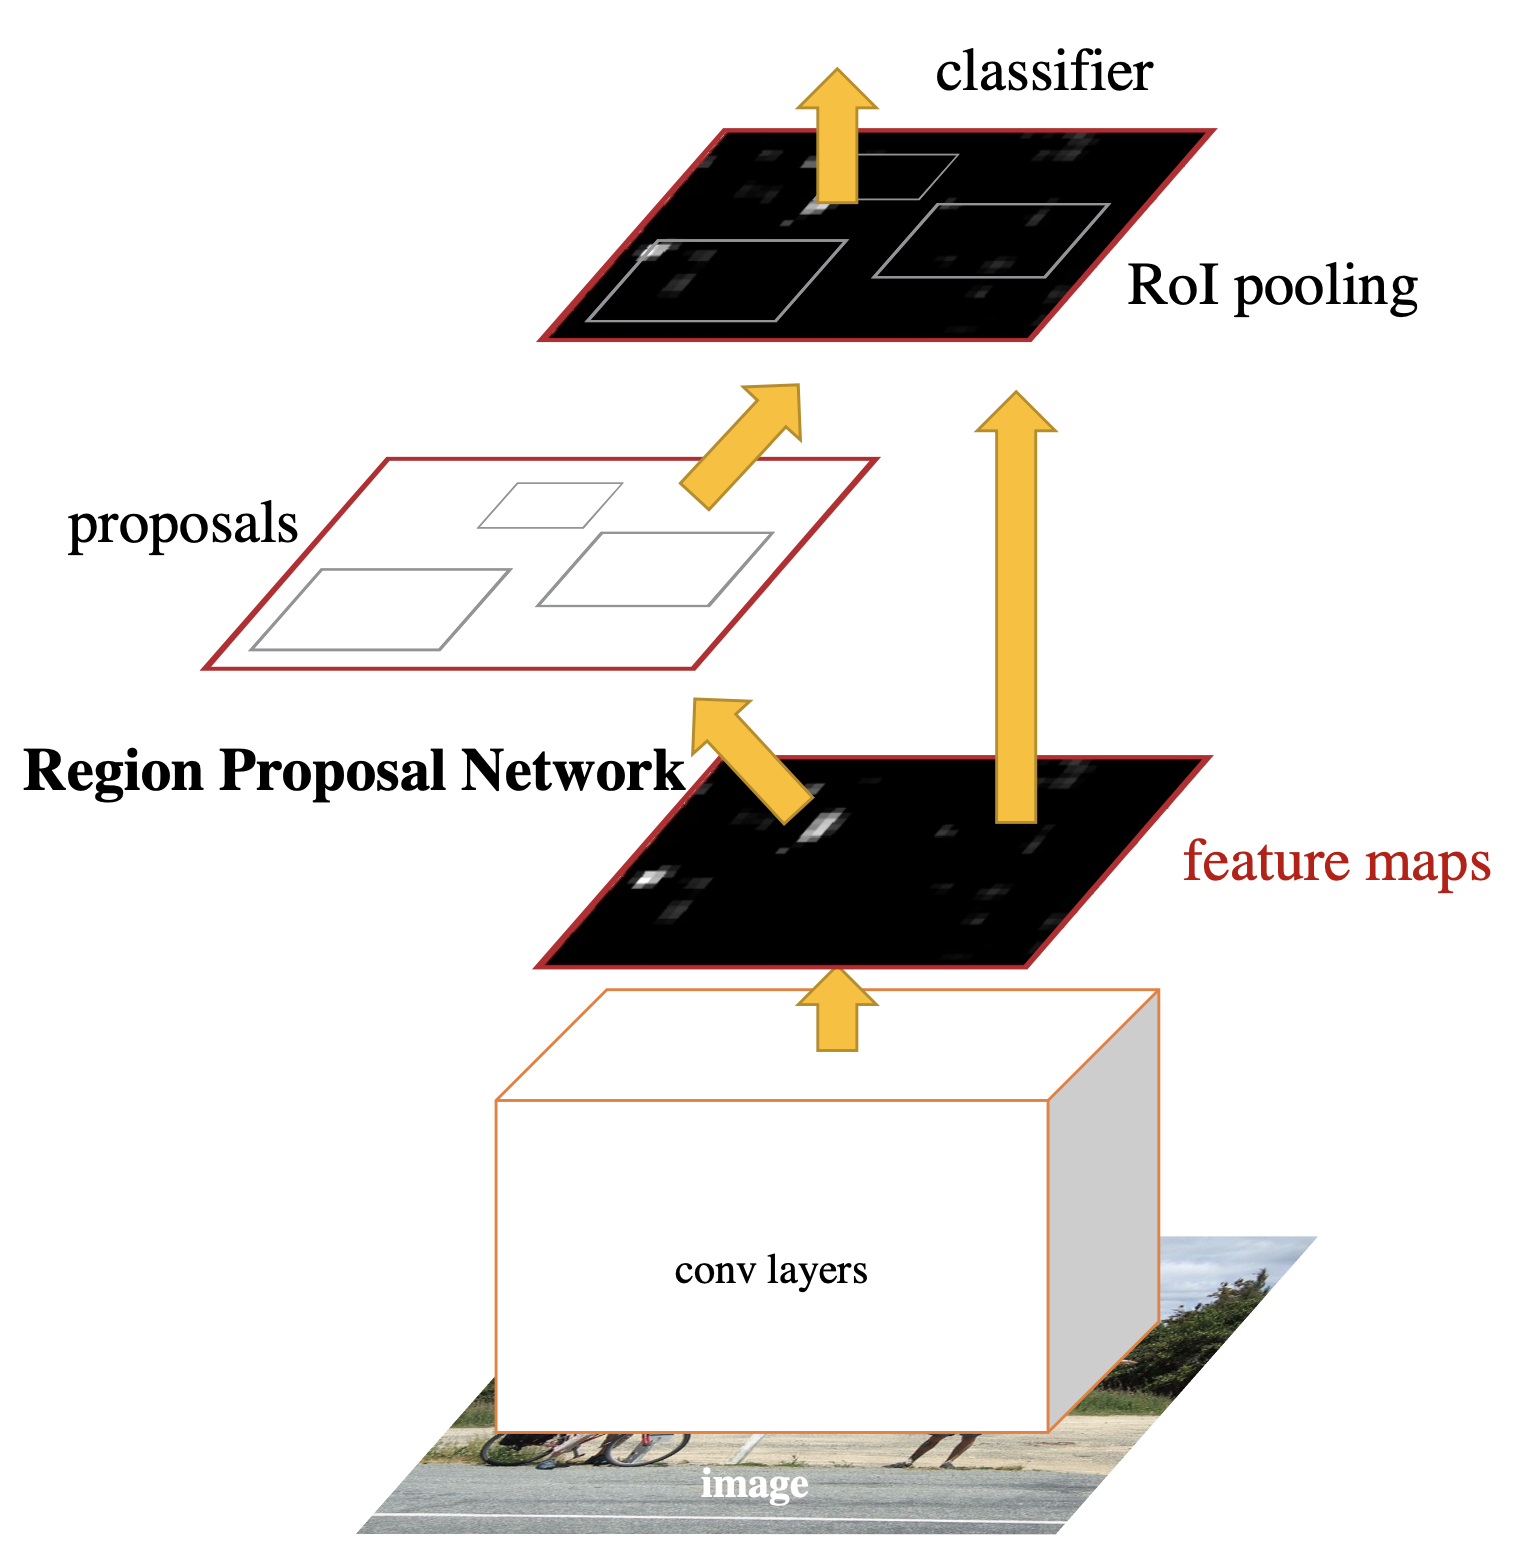
\includegraphics[height=5cm,keepaspectratio]{images/2_literature/faster-r-cnn.png}
\end{center}
\caption{Faster R-CNN: Object detection overview \cite{Ren2015}.}
\end{figure}


\subsubsection{YOLO}
The previous detectors all use regions to localize an object. The models look at parts of the image with high probability of containing an object. YOLO has a different architecture by looking at the complete image. A single neural network predicts bounding boxes and class probabilities in one evaluation. Using the system, you only look once (YOLO) at an image to see what objects it contains \cite{Redmon2016}.

YOLO as several benefits. First of all is that YOLO is extremely fast. Due the new architecture, it doesn't require a complex pipeline and can be trained end-to-end. Secondly, unlike previous models, YOLO reasons globally about the image. Most mistakes from top detector Fast R-CNN are due mistaking background for an object. YOLO makes less than half the number of background errors compared to Fast R-CNN. Finally, YOLO learns generalizable representations of objects. When trained on natural images and tested on art-work, YOLO outperforms top detectors such as R-CNN. 

YOLO does lag behind state-of-the-art detectors in accuracy. Although it can quickly detect objects, its struggles to precisely localize some objects, especially small ones. 

YOLO works by taking an image and split it into an SxS grid. Each grid predicts B bounding boxes and confidence scores for those boxes. These scores reflect how confident the model is that the box contains an object. The model outputs for each bounding box 5 predictions, the location (x, y), size (w, h) and confidence score. Additionally, each grid cell also predicts C conditional class probabilities. 

\begin{figure}[ht]
\begin{center}
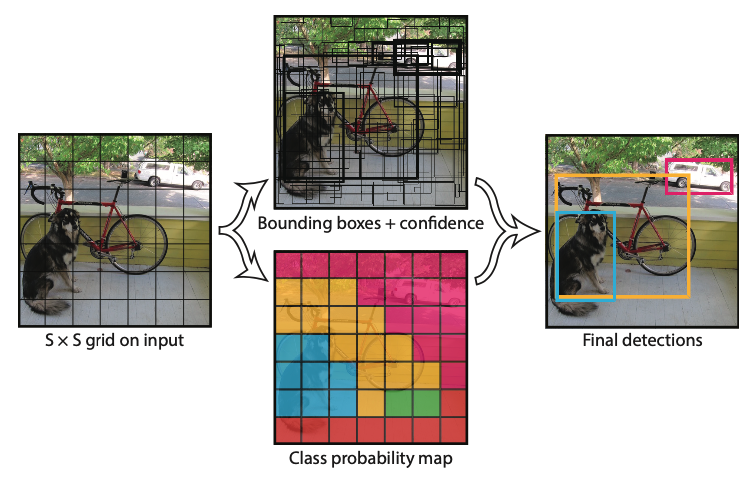
\includegraphics[width=10cm,keepaspectratio]{images/2_literature/yolo.png}
\end{center}
\caption{You Ony Look Once (YOLO) detector model \cite{Redmon2016}.}
\end{figure}


\subsubsection{YOLOv2}
The authors of YOLO continued their work and introduce two new detectors YOLOv2 and YOLO9000 \cite{Redmon2017}. They argue that current object detection datasets are limited (hundred thousand images) compared to datasets used for classification and tagging (millions of images with thousands of categories). They propose a novel method to harness large amount classification data and use it to expand current detection systems. Using this method they develop YOLO9000, a real-time object detector that can detect over 9000 categories. To do so, they first improve the base YOLO detection system to produce YOLOv2. 

YOLO suffers from various shortcomings relative to state-of-the-art detection systems. YOLO makes significantly number of localization errors compared to Fast R-CNN. Better performance often comes from training larger networks or ensambling networks together, instead the authors opt to simplify the network and introduce several architectural changes. In short, most improvements stem by applying state-of-the-art deep learning techniques, for details see \cite{Redmon2017}.  Below is shown an comparison of accuracy and speed between various detectors to demonstrate the effects.


\begin{figure}[ht]
\begin{center}
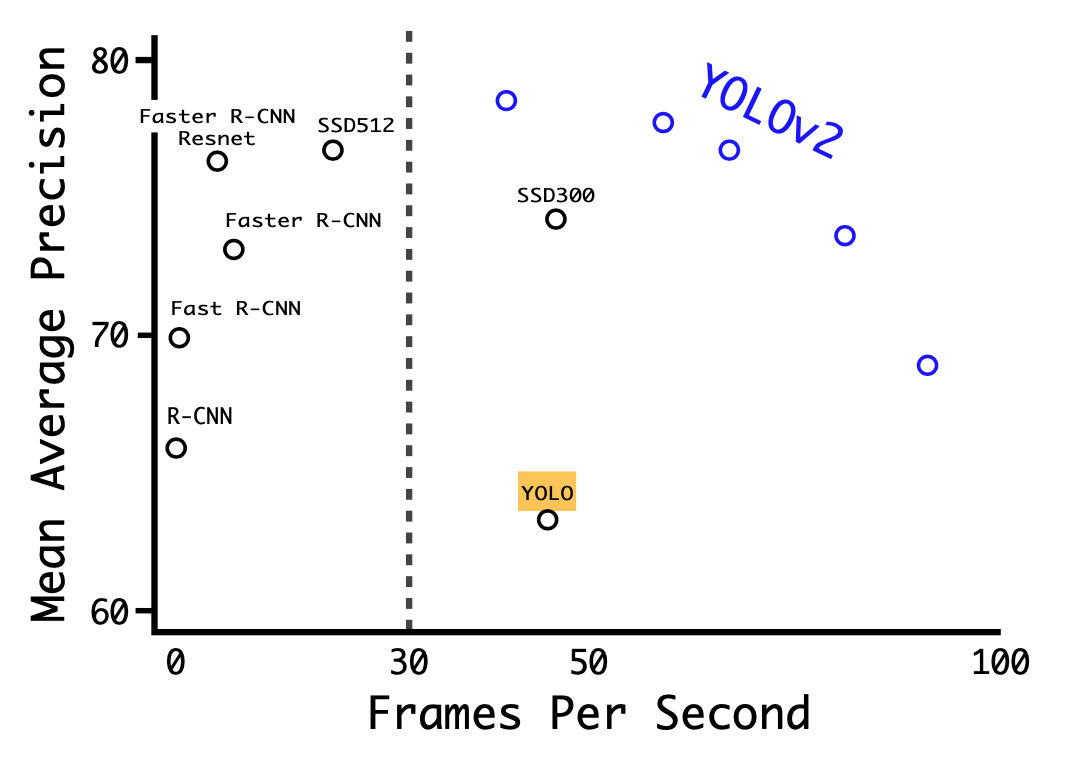
\includegraphics[width=10cm,keepaspectratio]{images/2_literature/yolov2-performance.png}
\end{center}
\caption{YOLOv2 accuracy and speed comparison on VOC 2007 \cite{Redmon2017}.}
\end{figure}

\subsubsection{YOLOv3}
YOLOv3 is another improved version of YOLO by the same authors \cite{Redmon2018}. It uses a new base model which is a bit slower but more accuracte. YOLOv3 predicts boxes at 3 different scales, based on the idea of Feature Pyramid Network \cite{Lin2017}. This allows the model to learn objects at different scales. Improving the performance of detecting smaller objects. Additionally, YOLOv3 performs multilabel classification instead of earlier used softmax.  Softmax asummes that labels are mutually exclusive, however it should be possible to classify an object as both woman and person. 


\begin{figure}[ht]
\begin{center}
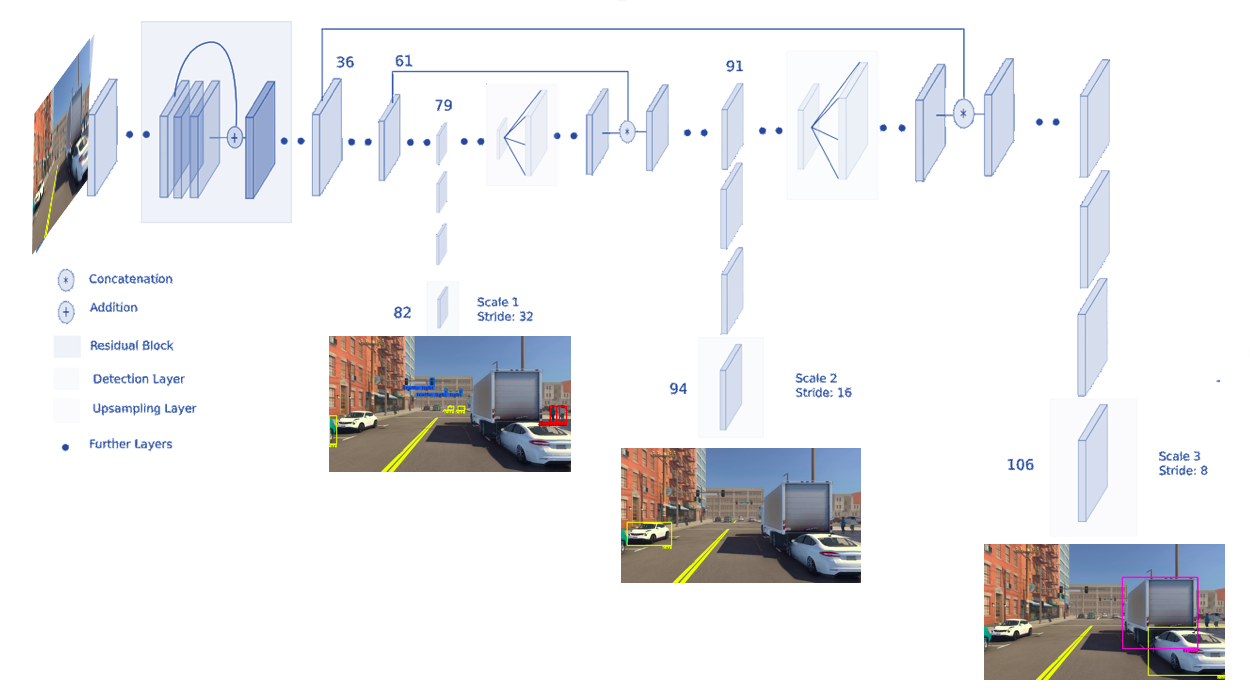
\includegraphics[width=14cm,keepaspectratio]{images/2_literature/yolov3-architecture.png}
\end{center}
\caption{YOLOv3 network architecture \cite{Dulepet2020}. Note that based on the output scale, the model detects objects of different sizes.}
\end{figure}


\subsubsection{YOLOv4}

YOLOv4 is the successor of YOLOv3. Unlike earlier models, YOLOv4 is developed by other authors \cite{Bochkovskiy2020}. In their paper the authors explore various deep learning techniques to improve the performance of YOLO, some deriving from earlier research, as well some novel techniques. The results is an improvement of 10\% accuraccy and about 12\% increase in speed.

One of these novel techniques is named Mosaic. It is a data augmentation method that mixes 4 training images. Thus 4 contexts are mixed. This allows detection of objects outside their normal context. In addition, batch normalization calculates statistics from 4 different images. Reducing the need for large mini-batch sizes.

Another novel technique is Self-Adversarial Training (SAT). This is also a data augmentation technique that operates in 2 stages. In the first stage, the network modifies the image instead of the weights. Thereby performing an adversarial attack on itself. In the second stage, the network is trained to detect an object on this modified image.


\subsubsection{YOLOv5}

Currently, there is no paper released on YOLOv5. At this time, it seems that YOLOv5 is still under active development \cite{Jocher2021}. Nevertheless, it has already been included in research \cite{Arya2020-competition}.


\subsubsection{Detection Transformers}

A complete different approach to object detection is DEtection TRansformers (DETR) \cite{Carion2020}. Transformers are deep learning architecture that recently gained popularity. They rely on powerful mechanism called attention, which enables the model to focus on certain parts of their input. 

\textit{TODO: To research further}


\subsubsection{Conclusion}


\subsection{Synchronization}
\label{section:synchronization}

In this thesis the aim is to fuse data of two modalities to perform road defects classification. Specifically, fusing visual and accelerometer data. In order to do so, the data streams need to be synchronized such that the same phenomena can be located in both sources. This is also referred to as alignment \cite{Baltrusaitis2017}.

Often in data fusion literature, modalities are misaligned due varying sampling rates, clock synchronization, or transmission delay between sensors. There are various known approaches to fix these issues. In general, the solution is designing a robust synchronization protocol to provide common notion of time. Existing methods often rely on a similarity measure or a trigger event between the different sources to fix this issue. Sensor synchronization is studied extensively in domain of sensor networks. When there is a similarity measure between the signals, the time delay between the signals can be calculated. To limit this review, research is only focused on synchronizing accelerometer and video data.

In order to compare video and accelerometer data, the key operation is to find a similarity measure between both sources. Conventionally, this is done by estimating acceleration from video movement \cite{Fridman2015,Zhang2020}. Estimating of accelerations can be done using the dense optical flow algorithm. It is computed as a function of two frames taken at time $t$ and $t + \Delta t$, where $\Delta t$ depends on the frame rate. The method to calculate optical flow is as follows. First, an estimate for the velocity for every pixel in adjacent frames is computed using Farneback algorithm \cite{Farnebäck2003}. The result is a 2D vector field, describing for each pixel the estimated motion in horizontal and vertical direction. By taking the average of all the estimated motions, a scalar acceleration is derived describing the acceleration of the frame.

To synchronize the accelerometer data with the visual data, the time delay needs to be computed. Note, that in our case this calculated delay refers to the $\tau_{caputure}$, refer back to section \ref{sec:relevance}. Cross correlation is a method often used to estimate the time delay between two signals \cite{Knapp1976}. Within the earlier research of \cite{Fridman2015, Zhang2020}, the authors also use cross correlation. Cross correlation is defined as.
\begin{align*}
R(\tau) = \int x(t) y(t + \tau) dt 
\end{align*}
Where $x(t)$ and $y(t)$ are the input signals, both a function of time, $\tau$ is the time delay, and R is the cross correlation, a function of time delay $\tau$. The optimal time shift for synchronizing both streams is computed by choosing the $\tau$ that maximizes the cross correlation. The original approach from \cite{Knapp1976} is rather expensive to compute and has a running time of $O(n^2)$. Fortunately, cross correlation can also be computed using more efficient FFT approach\cite{Lewis2001}. With a running time of $O(n \log n)$ \cite{Fridman2015}. Alternatively, optical flow can also be estimated using deep learning \cite{Deqing2017}, this approach is used in \cite{Zhang2020}.

TODO: Dynamic Time Warping

In this thesis synchronization of the sensors presents some challenges. Often it is sufficient to synchronize the capture time of the sensors. However in our case, the camera looks ahead, and we want to find the delay total $\tau = \tau_{capture} + \tau_{detection}$ between a detected object and when the vehicle travels over that object. This is challenging as, depending when the object is detected and the travelling speed, the detected object may be closer or father away. In theory, we could overcome this issue given the distance of the object to the vehicle and traveling speed. Calculating the distance of object to the vehicle is possible if we calibrate the visual signal. This calibration needs to be performed every time the smartphone is re-positioned. As it is unlikely that the smartphone is replaced consistently with the same angle at all times, a novel approach is developed in section \ref{sec:object-distance}.

\begin{figure}[ht]
\begin{center}
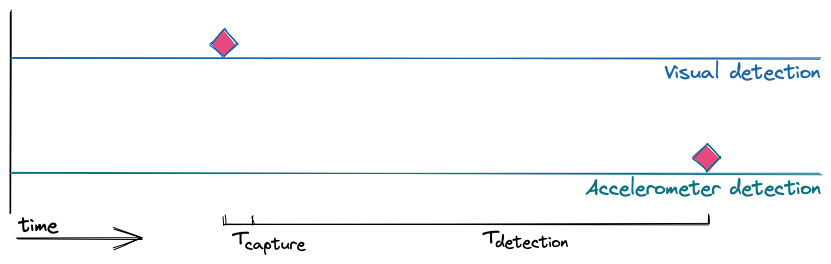
\includegraphics[width=0.95\textwidth,keepaspectratio]{images/2_literature/time-line-synchonization.png}
\end{center}
\captionsetup{width=0.95\textwidth}
\caption{Illustration of the synchronization problem: there is a delay between detecting the object and driving over that object.}
\end{figure}


Another key challenge for our data collection is partial observability. Partial observability refers to the fact that the same phenomena may not always be captured by both sensors. This happens because the field-of-view of the camera is much wider than that of the accelerometer. While the accelerometer can only detect a defect when the wheel of the vehicle travels over said defect. This is also visualized in figure \ref{fig:sensor-delay}.

\begin{figure}[ht]
\begin{center}
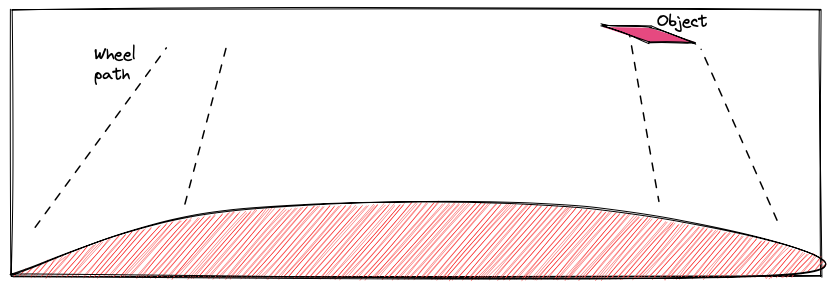
\includegraphics[width=0.95\textwidth,keepaspectratio]{images/2_literature/partial-observability.png}
\end{center}
\captionsetup{width=0.95\textwidth}
\caption{Illustration of the partial observability problem: objects in the accelerometer data can only be detected when the wheels of the vehicle drives over that object.}
\end{figure}



% When there is a similarity between the two data modalities, it is possible to align both streams 

% Cross correlation is a measure of similarity of two series as a function of the shift of one to the other.

% Learning from data often depends on cross correlation ...




% \subsection{Depth Estimation}




% The next challenge is that while driving, 

% The other method is to rely on 

% \textbf{Cross correlation}



% They use optical flow to capture fast ego-motion (i.e. vibration) for the front camera, and synchronize it with data from the accelerometer using cross correlation.

% One populair technique is Dynamic Time Warping (DTW). DTW measures the similarity between two sequences and finds the optimal match and inserts frames to align the time series.


% Most approaches to overcome this rely on a similarity measure between the modalities.  To overcome this, most approaches 



% \textbf{Cross correlation}

% \textbf{Dynamic Time Warping}

% \textbf{External trigger}
% One method to overcome this issue is using an external trigger to align the modalities. For instance in \cite{Cippitelli2015}, the authors are able to time synchronize visual data by calculating the delay when a controlled trigger is visible. 


% \subsection{Partial Observability}





% https://www.coursera.org/lecture/state-estimation-localization-self-driving-cars/lesson-2-multisensor-fusion-for-state-estimation-2imn3


\subsection{Signal Processing}

\subsubsection{Butterworth Filter}
\label{sec:butterworth-filter}

